\documentclass[12pt, a4paper] {article}
\usepackage[utf8]{inputenc}
\usepackage{graphicx}
\graphicspath{ {images/} }
\usepackage{amsmath}
\title{Assignment 1}
\author{Challa Akshay Santoshi- (CS21BTECH11012)}
\begin{document}
\maketitle
\textbf{\underline{ICSE 10 2018}}\\\\
\textbf{Question: 3 (c)}\\
Using a graph paper draw a histogram for the given distribution showing the number of runs scored by 50 batsmen. Estimate the mode of the data.\\\\
\setlength{\arrayrulewidth}{0.5mm}
\setlength{\tabcolsep}{18pt}
\renewcommand{\arraystretch}{1.5}
\begin{tabular}{ |p{2cm}|p{0.6cm}|p{0.6cm}|p{0.6cm}|p{0.6cm}|p{0.6cm}|p{0.6cm}|
p{0.6cm}|  }
\hline
Runs Scored & 3000-4000 & 4000-5000 & 5000-6000 & 6000-7000 & 7000-8000 & 8000-9000
& 9000-10000\\
\hline
No. of batsmen & 4 & 18 & 9 & 6 & 7 & 2 & 4 \\
\hline
\end{tabular}\\
\begin{center}
Table 1.1\\
\end{center}

\textbf{Solution: }\\\\
The Histogram for the data given in Table 1.1 is plotted as shown in Fig: 1.1. \\
The approach for calculating mode is outlined in Fig: 1.2. The interval corresponding to the maximum number of batsmen is the mode class. The intersection of the lines PQ and RS as shown in Fig 1.2 (Point M) is the mode point. The required mode is the x-coordinate of the Mode point.\\
\begin{center}
P =
$\begin{pmatrix}
  5000\\
  18
\end{pmatrix}$ 
Q =
$\begin{pmatrix}
  4000\\
  4\\
\end{pmatrix}$ 
\\
R =
$\begin{pmatrix}
  4000\\
  18
\end{pmatrix}$ 
S =
$\begin{pmatrix}
  5000\\
  9\\
\end{pmatrix}$ \\
\end{center}
Equations of lines are as follows:\\
\begin{align*} 
PQ : 14x - 1000y &=  52000 \\ RS : 9x + 1000y &=  54000 \\
\end{align*}
Adding both the equations, we get
\begin{align*}
23x &= 106000 \\
x &= 4068.695 \\
\end{align*}
From this we can get the y-coordinate as follows:
\begin{align*}
1000y &=  52000 + 14x \\
1000y &=  52000 + 56961.73 \\
y &= 12.521 \\
\end{align*}
Mode point is the point of intersection of lines PQ and RS.\\
Therefore mode point is\\
\begin{center}
M =
$\begin{pmatrix}
  4068.695\\
  12.521 
\end{pmatrix}$ 
\end{center}
Therefore, the mode is 4068.695.\\\\
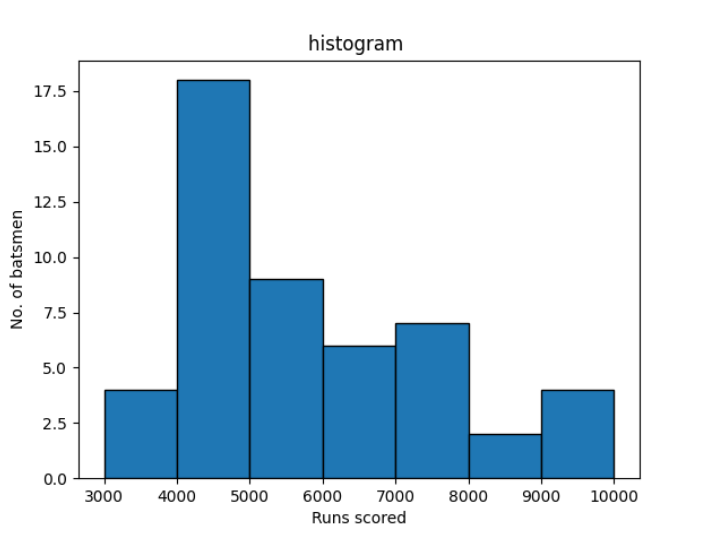
\includegraphics{fig 1.1}
\begin{center}
Fig: 1.1\\
\end{center}

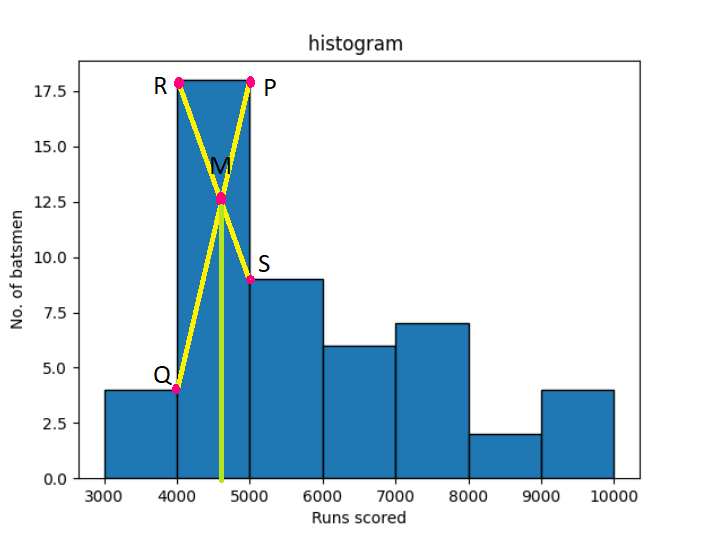
\includegraphics{fig 1.2}
\begin{center}
Fig: 1.2\\
\end{center}
\end{document}